%======================================================================
\chapter{Mechanism of \texorpdfstring{CO\textsubscript{2}}{CO2} Reduction}\label{chap.mech}
\markright{Computational Study of the Mechanism of \texorpdfstring{CO\textsubscript{2}}{CO2} Reduction}
%======================================================================

%======================================================================
\section{Literature Mechanisms}
%======================================================================

Literature has proposed three general mechanistic pathways for the photoreduction of \ce{CO2}. In general, as seen in \autoref{fig.threepath}, these pathways result in the formation of \ce{CO} and \ce{H2O}, formate (\ce{HCO2-}), or carbonate (\ce{COOH-}). The formation of \todo{carbonate or formate?} proceeds via the formation of a catalyst dimer over a molecule of \ce{CO2}, with the insertion of a second molecule of \ce{CO2} to produce the \todo{carbonate or formate} and a molecule of \ce{CO}. The formation of \ce{CO} without carbonate or formate byproducts occurs via the insertion of \ce{CO2} into a metal-hydride bond, followed by a proton addition and the release of a molecule of \ce{H2O} prior

\missingfigure{Three mechanistic pathway quick}
\begin{figure}[!htbp]
 \begin{center}
  \includegraphics[clip=true]{images/insertgraphic.eps}
 \end{center}
\caption[Overview of mechanistic pathways]{An overview of the mechanistic pathways of photochemical \ce{CO2} reduction}
\label{fig.threepath}
\end{figure} 
\todo{Make mechanism (or get morris?)}

%----------------------------------------------------------------------
\subsection{Subsection}
%----------------------------------------------------------------------

%----------------------------------------------------------------------
\subsection{Subsection}
%----------------------------------------------------------------------

%----------------------------------------------------------------------
\subsection{Subsection}
%----------------------------------------------------------------------

% - - - - - - - - - - - - - - - - - - - - - - - - - - - - - - - - - - - 
\subsubsection{SubSubSection}
% - - - - - - - - - - - - - - - - - - - - - - - - - - - - - - - - - - -

% - - - - - - - - - - - - - - - - - - - - - - - - - - - - - - - - - - -
\subsubsection{SubSubSection}
% - - - - - - - - - - - - - - - - - - - - - - - - - - - - - - - - - - -

% - - - - - - - - - - - - - - - - - - - - - - - - - - - - - - - - - - -
\subsubsection{SubSubSection}
% - - - - - - - - - - - - - - - - - - - - - - - - - - - - - - - - - - -
